%!TEX root = ../document.tex

\chapter{WLAN-Sicherheit}

\section{Erklärung}

In der folgenden Abbildung ist das Szenario so abgebildet, wie es in den meisten nachfolgenden
Angriffen angenommen wird. Es gibt ein Netzwerkgerät (Access Point), welches das Netzwerk
aufbaut und mindestens einen Client, der mit diesem Netzwerk verbunden ist. Wir befinden
uns in der Rolle des Angreifers und versuchen im Großteil der Anwendungsfälle Zugriff auf
das Netzwerk zu bekommen.
Angriffe auf ein Wireless Network laufen häufig nach einem bestimmten Schema ab. Dazu
werden Daten, die zwischen Client und Netzwerkgerät hin- und hergeschickt werden,
gesammelt. Diese Informationen werden dann beim Angreifer in einer gewissen Art und
Weise verarbeitet. Ist diese Verarbeitung, egal wie komplex diese ist, erfolgreich, so hat der
Angreifer häufig Zugriff auf das Netz.

\begin{figure}[H]
	\centering
	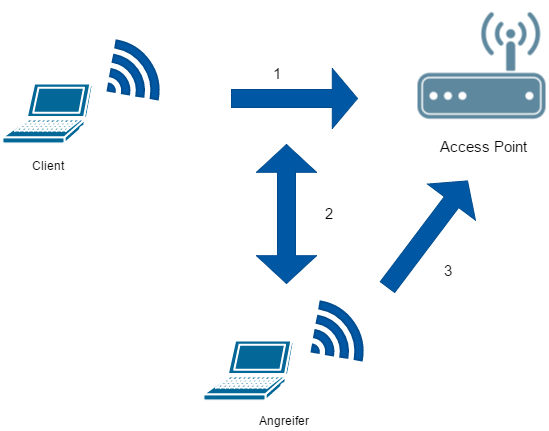
\includegraphics[width=0.8\textwidth]{images/WLAN/WLANSzenario.png}
	\caption{WLAN-Szenario}
	\label{fig:WLAN-Szenario}
\end{figure}

\section{Vorbereitung}

Voraussetzungen für die weiteren Übungen:

\begin{itemize}
	\item Alfa USB WLAN-Adapter, kann vom Labor bezogen werden
	\item WLAN-Router eingestellt auf das benötigte Verfahren (z.B. WEP,WPA), Archer C7 kann vom Labor bezogen werden
	\item Zwei Workstations/Notebooks
	\item Natives Kali Linux oder vom Labor bereitgestellter USB-Stick mit Kali Linux
	\item Grundlegende Kenntnisse mit Linux
\end{itemize}
Weitere Informationen zu der Hardware, die vom Labor bezogen werden kann, findet man in der nun folgenden Untersektion.

\section{Hardware}

\subsection{TP-Link Archer C7}
 Der WLAN-Router Archer C7 von TP-LINK eignet sich perfekt für die Verwendung bei den Tutorials der Security-Workbench. Dank simultanem Dualband kann der Router Übertragungsgeschwindigkeiten bis zu 450 Mbit/s auf 2,4GHz und bis zu 1300 Mbit/s auf 5GHz erreichen. Weitere Informationen findet man auf der Herstellerwebseite \url{http://www.tp-link.de/products/details/cat-9_Archer-C7.html}.

\begin{figure}[H]
	\centering
	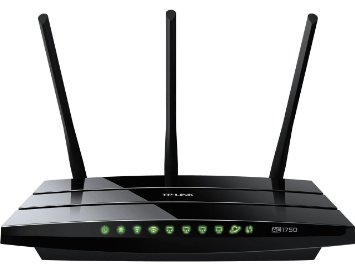
\includegraphics[width=0.5\textwidth]{images/WLAN/ArcherC7.jpg}
	\caption{Archer C7}
	\label{fig:Archer C7}
\end{figure}

\subsubsection{Betriebssystem und Software}
Der Archer C7 wird nicht mehr mit dem Originalbetriebssystem von TP-Link betrieben, stattdessen wird die freie Software OpenWrt in der Version 15.05 eingesetzt. Dies ermöglicht es, dass gleichzeitig mehrere WLAN-Netze mit verschiedenen SSIDs und Konfigurationen auf demselben WLAN-Interface des Router betrieben werden können. Dadurch können komfortabel alle Tutorials mit demselben Router durchgeführt werden, ohne diesen für jedes Tutorial erst konfigurieren zu müssen.\\
Zudem bietet OpenWrt die Möglichkeit von zusätzlichen Softwarepaketen. So kann beispielsweise Aircrack-ng auf dem Router installiert werden, gleiches gilt für FTP- oder HTTP-Server.

\subsubsection{Installation RADIUS-Server}
Besonders zu erwähnen ist die Möglichkeit einen RADIUS-Server für die Authentifikation in Enterprise-Netzen zu installieren. Da dies die Konfiguration mehrerer Pakete erfordert, folgt eine Kurzanleitung (Youtube Anleitung verfügbar unter \url{https://www.youtube.com/watch?v=PvUqMFvTOn8)}):
\begin{enumerate}
	\item {Update des Softwarecenters}\\
	\colorbox{altgray}{\lstinline|opkg update|}
	\item {Entfernen des Standard WLAN-Pakets}\\
	\colorbox{altgray}{\lstinline|opkg remove wpad-mini|}
	\item { Installation eines mächtigeren WLAN-Deamons}\\
	Der Deamon wird benötigt, um WPA/WPA2-Netze mit RADIUS-Server-Authentifikation zu erstellen. \\
	 \colorbox{altgray}{\lstinline|opkg install wpad|}
	\item {(Optional:) Installation eines Texteditors}\\ \colorbox{altgray}{\lstinline|opkg install nano|}
	\item {Installation von Freeradius2-Komponenten}\\
	\colorbox{altgray}{\lstinline|opkg install [Pakete]|}:\\
	Schritt 1: Installation von\\
	\textit{freeradius2 freeradius2-mod-always freeradius2-mod-attr-filter freeradius2-mod-attr-rewrite freeradius2-mod-chap freeradius2-mod-detail freeradius2-mod-eap freeradius2-mod-eap-gtc freeradius2-mod-eap-md5 freeradius2-mod-eap-mschapv2 freeradius2-mod-eap-peap freeradius2-mod-eap-tls freeradius2-mod-eap-ttls freeradius2-mod-exec freeradius2-mod-expiration freeradius2-mod-expr freeradius2-mod-files freeradius2-mod-ldap freeradius2-mod-logintime freeradius2-mod-mschap freeradius2-mod-pap}\\
	Schritt 2: Installation von\\
	\textit{freeradius2-mod-passwd freeradius2-mod-preprocess freeradius2-mod-radutmp freeradius2-mod-realm freeradius2-mod-sql freeradius2-mod-sql-mysql freeradius2-mod-sql-pgsql freeradius2-mod-sql-sqlite freeradius2-mod-sqlcounter freeradius2-mod-sqllog freeradius2-utils freeradius2-democerts}
	\item {Wechsel in das Verzeichnis \colorbox{altgray}{\lstinline|/etc/freeradius2/|}}\\
	\colorbox{altgray}{\lstinline|cd /etc/freeradius2/|}
	\item {Editieren der Userkonfiguration: \colorbox{altgray}{\lstinline|nano users|}}\\
	Anlegen eines neuen Nutzers am Ende der Datei: \textit{username Cleartext-Password := "Password"}
	\item {Editieren der Clientkonfiguration: \colorbox{altgray}{\lstinline|nano clients.conf|}}
	\begin{itemize}
		\item Im Abschnitt \textit{Client localhost} anpassen der \textit{ipaddr = 127.0.0.1} auf Router-IP.
		\item Anpassen des \textit{secrets = testing123} (Bei der Erstellung eines Enterprise-APs anzugeben)
	\end{itemize}

	\item {Editieren der Serverkonfiguration: \colorbox{altgray}{\lstinline|nano radiusd.conf|}}
	\begin{itemize}
		\item Unter \textit{listen} die Zeile \textit{interface = br-lan} auskommentieren.
		\item Unter \textit{logs} den Wert von  \textit{auth = } auf \textit{yes} setzen.
	\end{itemize}

	\item {Installieren von Openssl} \\
	\colorbox{altgray}{\lstinline|opkg install openssl-util|}
	\item {Löschen der Demozertifikate}
	\begin{itemize}
		\item Wechsel in das Verzeichnis \textit{certs}: \colorbox{altgray}{\lstinline|cd /etc/freeradius2/certs|}
		\item \colorbox{altgray}{\lstinline|rm ca.pem|}
		\item \colorbox{altgray}{\lstinline|rm server.pem|}
	\end{itemize}

	\item {Erstellen einer neuen CA und eines Serverzertifikats}\\
	Es können beliebige Daten bei den Zertifikaten verwendet werden. Die verwendeten Passwörter werden später benötigt. Falls ein Challenge-Passwort gefordert wird, ist das Feld leer zulassen. \\
	\textit{ACHTUNG:} Unterschiedliche Common Names bei CA- und Serverzertifikat angeben.
	\begin{itemize}
		\item \colorbox{altgray}{\lstinline|openssl genrsa -des3 -out ca.key 2048|}
		\item \colorbox{altgray}{\lstinline|openssl req -new -x509 -days 9999 -key ca.key -out ca.pem|}
		\item \colorbox{altgray}{\lstinline|openssl genrsa -des3 -out server.key 2048|}
		\item \colorbox{altgray}{\lstinline|openssl req -new -key server.key -out server.csr|}
		\item \colorbox{altgray}{\lstinline|openssl x509 -req -days 9999 -in server.csr -CA ca.pem|} \\  	 \colorbox{altgray}{\lstinline|-CAkey ca.key -set_serial 01 -out server.pem|}
	\end{itemize}


	\item {Wechsel nach \colorbox{altgray}{\lstinline|/etc/freeradius2/|} }\\
	\colorbox{altgray}{\lstinline|cd /etc/freeradius2/|}
	\item {Editieren der EAP-Konfiguration: \\
	\colorbox{altgray}{\lstinline|nano eap.conf|}}
	\begin{itemize}
		\item Unter \textit{tls} bei \textit{private\_key\_password} das Passwort aus der Keyerstellung angeben.
		\item \textit{private\_key\_file} Name des Keys anpassen auf \textit{server.key}
	\end{itemize}

	\item {Reboot des Routers} \\
	\colorbox{altgray}{\lstinline|reboot|}
	\item {Enable und Start des Servers}
	\begin{itemize}
		\item \colorbox{altgray}{\lstinline|/etc/init.d/radiusd enable|}
		\item \colorbox{altgray}{\lstinline|/etc/init.d/radiusd start|}
	\end{itemize}

\end{enumerate}
Nach Durchführung der Installation und Konfiguration kann in der Weboberfläche des Routers ein Enterprise-AP erstellt werden und es müssen die IP des Routers und das festgelegte Secret angegeben werden.

\subsubsection{Eingerichtete WLAN-Netze und Passwörter}
Für die Anmeldung auf der Routeroberfläche wird folgender Login benötigt:
\begin{itemize}
	\item User: \textit{root}
	\item Passwort: \textit{toor}
\end{itemize}
Nachfolgend werden alle eingerichteten WLAN-Netze mit den dazugehörigen Keys/PSKs aufgelistet:
\begin{enumerate}
	\item {WEP}
	\begin{itemize}
			\item HackMe\_WEP\_Open: BC6AFE583E
			\item HackMe\_WEP\_Shared: BC6AFE583E
			\item HackMe\_WEP\_Open\_5GHz: BC6AFE583E
			\item HackMe\_WEP\_Shared\_5GHz: BC6AFE583E
	\end{itemize}
	\item {WPA}
	\begin{itemize}
		\item HackMe\_WPA: HackMeHa
		\item HackMe\_WPA2: HackMeHa
		\item HackMe\_DoS: HackMeHa
		\item HackMe\_WPA\_5GHz: HackMeHa
		\item HackMe\_WPA2\_5GHz: HackMeHa
		\item HackMe\_DoS\_5GHz: HackMeHa
	\end{itemize}
\end{enumerate}

\subsection{Alfa AWUS051NH 802.11abgn USB Adapter Dual-Band 2.4GHz/5GHz}

Der Alfa Adapter sollte grundsätzlich über Plug and Play unter Kali funktionieren. Er eignet sich als leistungsstarke externe USB-WLAN Karte für die hier durchgeführten Versuche. Der Adapter ist sowohl kompatibel mit aktuellen Verfahren wie WPA und WPA2, als auch mit veralteten Verfahren wie WEP. Er lässt sich mit Windows, Mac OS und gängigen Linux Distributionen verwenden.
Weitere Informationen findet man auf der Herstellerwebseite unter \url{https://www.alfa.com.tw/products_show.php?pc=67&ps=241}.

\begin{figure}[H]
	\centering
	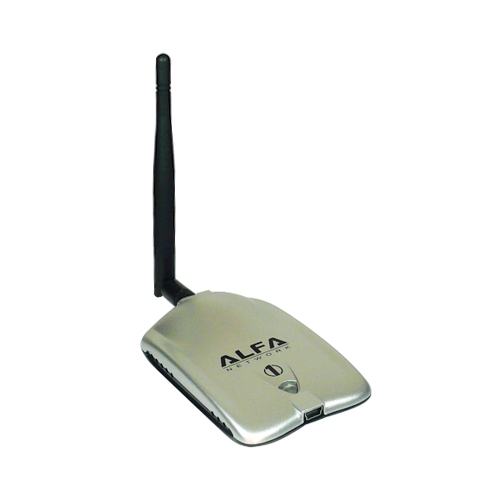
\includegraphics[width=0.5\textwidth]{images/WLAN/AlfaUSB-Adapter.jpg}
	\caption{Alfa USB-Adapter}
	\label{fig:Alfa USB-Adapter}
\end{figure}
\newpage

\section{WEP}

WEP (Wired Equivalent Privacy) ist ein Standard für die Verschlüsselung und Authentifizierung
von WLANs aus dem Jahr 1999. Ziel war es, Funknetzwerke genauso sicher, wie kabelgebundene Netzwerke zu machen. Um dieses Ziel zu erreichen, bietet WEP Mechanismen für die Authentifizierung, Verschlüsselung und Integritätsprüfung. WEP enthält grundlegende Design-Schwächen und gilt seit 2001 als geknackt. Die Berechnung des Schlüssels aus einigen Minuten an aufgezeichneten Daten dauert normalerweise nur wenige Sekunden. Daher sollten WLAN-Installationen die sicherere WPA2-Verschlüsselung verwenden.

\subsection{Unterschied von Open System Authentication und Shared Key Authentication}

Für die Authentifizierung der Clients am Access Point sieht WEP zwei Varianten vor, die Open System Authentication oder die Shared Key Authentication.

	\subsubsection{Open System Authentication}
	Die Open System Authentication ist die Standard-Authentifizierung bei WEP. Die Open System Authentication ist die Standard-Authentifizierung.

	Ist der Accesspoint für keine Verschlüsselung konfiguriert, findet praktisch keine Authentifizierung statt und jeder Client kann sich mit dem WLAN verbinden.
	Ist der Accesspoint für Verschlüsselung konfiguriert (in diesem Fall WEP), gibt es zwei Arten: \\
	\begin{itemize}
	\item Logisch: Der WEP-Schlüssel dient gleichzeitig zur Authentifizierung und jeder Client mit korrektem WEP-Schlüssel bekommt Zugang zum Netz.

	\item Technisch: Es findet ein Austausch von Authentifizierungsnachrichten statt und der Client wird authentifiziert. Stimmen WEP-Key auf Accesspoint und Client überein, ist Kommunikation möglich. Stimmen diese nicht überein, ist der Client zwar authentifiziert, kann jedoch keine Daten mit dem Netz austauschen. \\
	\end{itemize}

	\subsection{Shared Key Authentication}
	Die Shared Key Authentication setzt das WLAN-Passwort zur Authentifizierung der WLAN Clients ein. Die Authentifizierung erfolgt per Challenge-Response-Verfahren. Das bei WEP verwendete Verschlüsselungsverfahren ist RC4, eine Datenstromchiffrierung. \\
		\begin{figure}[H]
			\centering
			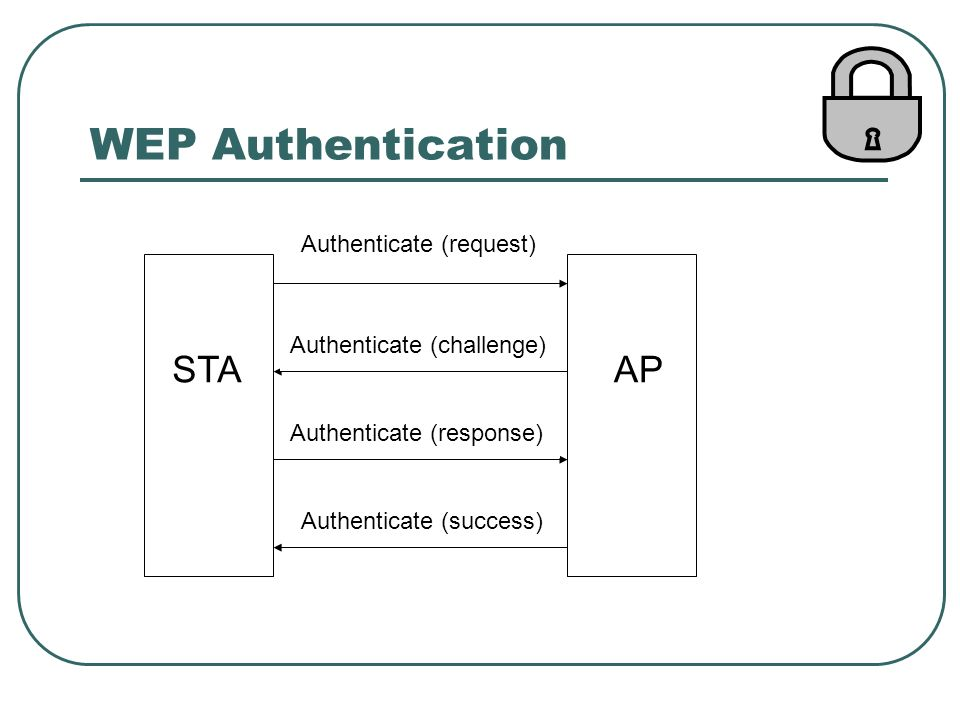
\includegraphics[width=0.8\textwidth]{images/WLAN/WEPchres.jpg}
			\caption{Challenge/Response bei WEP}
			\label{fig:Challenge/Response bei WEP}
		\end{figure}
	Nach der Authentifizierung und Verbindung wird der zuvor ausgetauschte WEP-Schlüssel für die Verschlüsselung der Daten mit RC4 verwendet. Im ersten Moment erscheint die shared-Variante sicherer als die open-Variante, da diese keine Authentifizierung anbietet. Das ist allerdings irreführend, da es ist möglich, den Vorgang des Schlüsselaustauschs abzuleiten, der für den Handshake verwendet wird, indem er die Challenge-Frames in der Shared Key-Authentifizierung erfasst. Sollte also die Privatsphäre ein entscheidender Punkt sein, wäre es ratsamer die open-Variante zu nutzen. Allerdings sei hier noch einmal darauf hingewiesen, dass beide Verfahren als schwach zu bezeichnen sind.

	\subsection{WEP-Verschlüsselung}

	Das WEP-Protokoll verwendet den RC4-Algorithmus als Pseudozufallszahlengenerator (PRNG) bei der Erzeugung eines Keystreams, der einen Schlüssel und einen Initialisierungsvektor (IV) als Eingabe erhält. Für jede zu schützende Nachricht M wird ein neuer 24 Bit langer Initialisierungsvektor gebildet und mit einem Schlüssel K verknüpft, der allen Stationen im WLAN bekannt ist. Das Ergebnis dient als Eingabe für den RC4-Algorithmus, welcher daraus einen Keystream erzeugt. Zusätzlich wird mittels Zyklischer Redundanzprüfung (ZRP, engl. CRC) ein vermeintlich sicherer „Integritätsprüfwert“ (Integrity Check Value – ICV) berechnet und an die Nachricht M angehängt (||). Die resultierende Nachricht (M||ICV) wird mit dem Keystream (RC4(IV||K)) des RC4-Algorithmus XOR-verknüpft und der Initialisierungsvektor IV wird dem resultierenden Ciphertext vorangestellt. Die unteren Abbildungen verdeutlichen Verschlüsselung und Entschlüsselung.

	\begin{figure}[H]
		\centering
		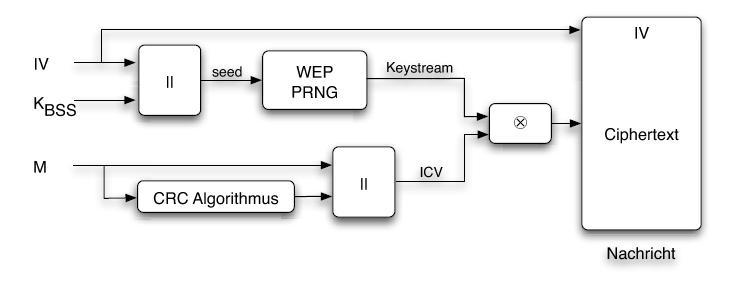
\includegraphics[width=0.9\textwidth]{images/WLAN/WEPKodierung.JPG}
		\caption{WEP Verschlüsselung}
		\label{fig:WEP Verschlüsselung}
	\end{figure}

	\begin{figure}[H]
		\centering
		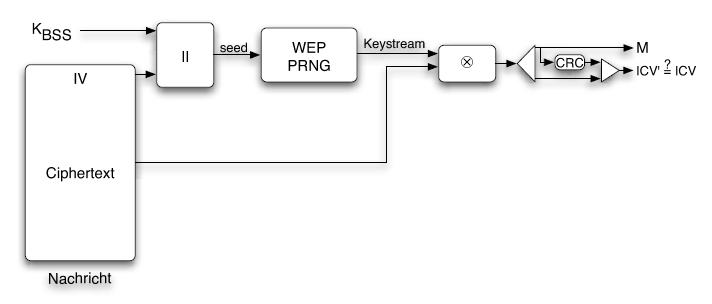
\includegraphics[width=0.9\textwidth]{images/WLAN/WEPDekodierung.JPG}
		\caption{WEP Entschlüsselung}
		\label{fig:WEP Entschlüsselung}
	\end{figure}

	Ein mit WEP verschlüsseltes Datenpaket besteht aus dem geheimen WEP-Schlüssel mit 40 oder 104 Bit Länge (WEP64 / WEP128), einer 32 Bit Prüfsumme der unverschlüsselten
	Daten und, wie oben bereits erwähnt, einem 24 Bit langem Initialisierungsvektor, den WEP-Schlüssel zum Gesamtschlüssel auf 64 Bit oder 128 Bit verlängert und einmal pro
	Datenpaket inkrementiert (-1) wird. \\
	Das gesamte Datenpaket besteht aus den Daten und der 32 Bit-Prüfsumme. Dies wird
	mit der IV-WEP-Schlüssel-Kombination verschlüsselt.

			\begin{figure}[H]
				\centering
				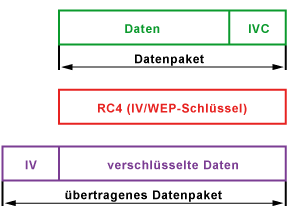
\includegraphics[width=0.7\textwidth]{images/WLAN/WEPpakete.png}
				\caption{WEP Pakete}
				\label{fig:WEP Pakete}
			\end{figure}

\subsection{Schwächen bei WEP}
Der IV wird bei jedem Frame fortlaufend inkrementiert, weshalb er irgendwann wiederholt
wird. Da der IV im Klartext übertragen wird, entspricht die effektive Verschlüsselung nur 40 bzw. 104 Bit, obwohl häufig von 64 oder 128 Bit gesprochen wird. Die Authentifizierung, Verschlüsselung und Integritätsprüfung verwenden zudem den gleichen Schlüssel. \\
Ein Angriff auf die WEP-Verschlüsselung erfolgt üblicherweise durch das Aufzeichnen einer
ausreichenden Menge an Datenverkehr. Außerdem muss sich in diesem Zusammenhang auch jemand in dem WLAN befinden, dass gehackt werden soll, um das Verbinden mit dem Access Point aufzunehmen.
Aus dem aufgenommenen Verkehr lässt sich im Anschluss daran der WEP-Schlüssel berechnen. Dies geschieht durch das Aufzeichnen der $2^{24}$ Schlüsselmöglichkeiten des IV, welche aufgrund der inkrementierenden Zählweise irgendwann wiederholt werden müssen. Bei einem durchschnittlich ausgelasteten Access Point sind die Datenpakete auf circa eine Stunde gesammelt. Allerdings ist es möglich, diesen Vorgang zu beschleunigen. \\
\\
\subsubsection{Theoretischer Aufbau eines WEP-Hacks}
\begin{enumerate}
	\item Vorbereiten des Netzwerkinterfaces
	\item Aktivieren des Monitoring-Mode
	\item WLAN mit WEP identifizieren
	\item Datenverkehr mit Airodump-ng aufzeichnen
	\item Authentifizierung am AP und generieren von Datenverkehr (optional)
	\item Errechnen des WEP-Kennworts
\end{enumerate}
Die genaue Beschreibung des Vorgangs wird im folgenden Punkt beschrieben.

\subsection{Cracking der WEP-Verschlüsselung}

	\subsubsection{Vorbereiten des Netzwerkinterfaces}
	Über den Befehl \colorbox{altgray}{\lstinline|ifconfig|} lässt sich erkennen, ob der WLAN-Adapter vom Host korrekt erkannt und initialisiert wurde. Dieser taucht normalerweise als \colorbox{altgray}{\lstinline|wlanX|} in der angezeigten Liste auf. Des Weiteren wird hier auch die MAC-Adresse des Adapters angezeigt. Beides wird im weiteren Verlauf noch benötigt.
	Anschließend muss die Netzwerkkarte einsatzbereit gemacht werden. Hierzu ist es nötig, eventuell
	störende Prozesse auf dem Host zu beenden. Hierzu wird ein Terminal geöffnet und der
	Befehl \colorbox{altgray}{\lstinline|airmon-ng check kill|} eingegeben.

	\subsubsection{Identifikation des Ziel-Netzwerks}
	Im nächsten Schritt identifizieren wir das WLAN, welches angegriffen werden soll. Der Befehl \colorbox{altgray}{\lstinline|airodump-ng wlanX|} gibt eine Liste mit in der Umgebung verfügbaren Netzwerken aus. Das X sollte durch die im ersten Schritt identifizierte Nummer des Interfaces ersetzt werden.
	Dabei wir das Interface automatisch in den Monitoring-Mode versetzt. Aus der angezeigten Liste wählen wir das entsprechende WLAN aus. Für später benötigen
	wir dabei die Art der Authentifizierung, den Netzwerknamen oder SSID, den Kanal und die BSSID oder Mac-Adresse des
	Ziels.

	\subsubsection{Cracking der Shared Key Authentication}
	Folgendes Kapitel ist nur relevant wenn das anzugreifende Netzwerk mit der Shared Key Authentication Variante von WEP gesichert ist. Für das Knacken von WEP-Shared-gesicherten Netzen muss eine Deauthentication vom AP vermieden werden. \\
	Für die Lösung dieses Problem bietet \colorbox{altgray}{\lstinline|aircrack-ng|} die Möglichkeit zur Erstellung eines PRGA (pseudo random generation algorithm) xor files wodurch eine Fake Authentication möglich wird. Der Vorgang wird nun beschrieben:

	\begin{enumerate}
		\item Start des Monitor Mode \\
		 Im ersten Schritt starten wir den Monitor Mode mit dem Befehl: \\ \colorbox{altgray}{\lstinline|airmon-ng start wlanX|}

		\item Erstellen eines PRGA-Files \\
		Starten von airodump-ng um ein PRGA-File anzulegen. Es muss gewartet werden bis eine Shared-Key-Authentication (SKA) aufgenommen wurde.\\
		\colorbox{altgray}{\lstinline|airodump-ng -c KANAL --bssid BSSID -w sharedkey wlanX|} \\
		\begin{itemize}
			\item -c spezifiziert den Kanal des WLANs
			\item Auf --bssid folgt die BSSID des Ziels
			\item -w sharedkey definiert das Präfix der PRGA xor Datei, dass für die Fake Authentication notwendig ist

			\item wlanX ist der Name des eigenen WLAN-Adapters
		\end{itemize}
		Die Aufnahme sieht wie folgt aus. Dabei ist zu beachten, dass unter AUTH das SKA erscheint wenn eine Shared-Key-Authentication (SKA) aufgenommen wurde erst dann ist der Vorgang erfolgreich.
		\begin{figure}[H]
			\centering
			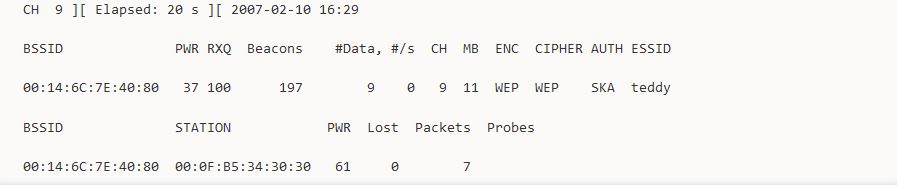
\includegraphics[width=0.9\textwidth]{images/WLAN/beispielSKA.JPG}
			\caption{SKA-Aufnahme}
			\label{fig:SKA-Aufnahme}
		\end{figure}

		Nach der erfolgreichen Aufnahme befinden sich drei neue Dateien im Verzeichnis. Beispiele für die drei Dateien zeigt folgende kleine Abbildung. Relevant für den nächsten Schritt ist die \colorbox{altgray}{\lstinline|sharedkey.xor|} Datei. Mit der Datei kann die Fake Authentication durchgeführt werden.

		\begin{figure}[H]
			\centering
			\includegraphics[width=0.9\textwidth]{images/WLAN/sharedBSP.JPG}
			\caption{Sharedkey Files}
			\label{fig:Sharedkey Files}
		\end{figure}

		\item Durchführen einer Shared-Key-Fake-Authentication \\
		Der folgende Befehl wird benutzt um die Shared-Key-Fake-Authentication durchzuführen und damit das Cracken des WEP-Shared gesicherten Netzes zu ermöglichen. \\
		\colorbox{altgray}{\lstinline|aireplay-ng -1 0 -e SSID -y sharedkey.xor -a BSSID -h WLAN-MAC wlanX|} \\
		\begin{itemize}
				\item -1 bedeuted, dass ein fake authentication durchgeführt wird und 0 steht für eine einmalige Authentication.
				\item -e spezifiziert die SSID des Ziels
				\item -y sharedkey.xor ist der Name der Datei die die PRGA xor bits enthält
				\item -a spezifiziert die BSSID des Ziels
				\item -h spezifiziert die BSSID des eignen WLAN-Adapters
				\item wlanX ist der Name des eigenen WLAN-Adapters
		\end{itemize}
		Sollte der Vorgang erfolgreich gewesen sein müsste folgende Ausgabe zu sehen sein:

		\begin{figure}[H]
			\centering
			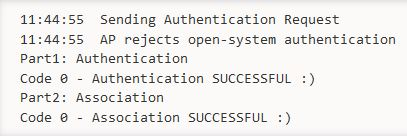
\includegraphics[width=0.7\textwidth]{images/WLAN/sharedSuccess.JPG}
			\caption{Fake Authentication Success}
			\label{fig:Fake Authentication Success}
		\end{figure}

		\item Stop des Monitor Mode \\
		 Abschließend stoppen wir den Monitor Mode mit dem Befehl, da wir ihn im nachfolgenden Szenario nicht mehr benötigen. \\
		 \colorbox{altgray}{\lstinline|airmon-ng stop wlanX|} \\
		 Das WEP-Cracking-Verfahren wird im nächsten Kapitel fortgeführt. Ab dem nächsten Schritt unterscheidet sich das Cracking von der Open und Shared Variante von WEP nicht mehr.

	\end{enumerate}

	\subsubsection{Aufzeichnen der WLAN Pakete mit airodump}
	Nun muss der Netzwerkverkehr im Zielnetzwerk aufgezeichnet erden. Dies erledigt das
	Werkzeug airodump mit folgendem Befehl: \\
	\colorbox{altgray}{\lstinline|airodump-ng -c KANAL -w SSID --bssid BSSID wlanX|}
	Die Pakete werden in einem .cap-File aufgezeichnet, welches im aktuellen Verzeichnis angelegt wird.
	\begin{itemize}
		\item -c spezifiziert den Kanal des WLANs
		\item -w spezifiziert die SSID des Ziels
		\item Auf --bssid folgt die BSSID des Ziels
		\item wlanX ist der Name des eigenen WLAN-Adapters
	\end{itemize}
	\subsubsection{Injection Test auf das Zielnetzwerk}
	An dieser Stelle testen wir mit folgendem Befehl, ob das Ziel angreifbar ist: \colorbox{altgray}{\lstinline|aireplay-ng -9 -e SSID -a BSSID wlanX|}
		\begin{itemize}
			\item -9 definiert einen Injection Test mit \colorbox{altgray}{\lstinline|aireplay-ng|}
			\item -e spezifiziert die SSID des Ziels
			\item -a spezifiziert die BSSID des Ziels
			\item wlanX ist der Name des eigenen WLAN-Adapters
		\end{itemize}

	\subsubsection{Generieren von zusätzlichem Datenverkehr auf dem Access Point}
	Um die für einen erfolgreichen Angriff benötigte Datenmenge schnell zu erreichen, gibt es die
	Möglichkeit authentication-Pakete in das Netzwerk einzuschleusen. Dabei kann der Angriff auf das
	Netzwerk allerdings entdeckt werden. Zunächst öffnen wir ein neues Terminal. Anschließend authentifizieren wir uns mithilfe des Tools \colorbox{altgray}{\lstinline|aireplay-ng|} am Access Point mit dem Befehl \colorbox{altgray}{\lstinline|aireplay-ng - 1 6 -o 1 -q 1 -e SSID -a BSSID -h WLAN-MAC wlanX|}
			\begin{itemize}
				\item - 1 6 steht für den fake authentication-modus, bei dem sich alle 6 Sekunden wieder authentifiziert wird
				\item -h spezifiziert die BSSID des eigenen WLAN-Adapters
				\item -e spezifiziert die SSID des Ziels
				\item Mit -o 1 wird veranlasst nur eine Ladung von Paketen auf einmal zu versenden. Der Defaultwert ist die mehrfach Sendung von Paketen was manche Access Points verwirren kann
				\item -a spezifiziert die BSSID des Ziels
				\item -q 1 sendet jede Sekunde eine keep-alive-Nachricht
				\item wlanX ist der Name des eigenen WLAN-Adapters. Dies ist nötig, da der Access Point sonst die injizierten Pakete verwirft und keinen verwertbaren Datenverkehr zurückliefert.
			\end{itemize}

	\subsubsection{Lauschen auf ARP-Requests und injizieren ins Ziel}
	Anschließend lauschen wir auf ARP-Requests anderer Teilnehmer im Netzwerk, was natürlich nur entstehen kann, wenn sich andere Teilnehmer im Zielnetzwerk befinden, und - wenn
	genügend zusammen gekommen sind - injizieren wir diese ins Netzwerk mit \colorbox{altgray}{\lstinline|aireplay-ng -3 -b BSSID -h WLAN-MAC wlanX|}.
	Die Anzahl an aufgezeichneten Datenpaketen im ersten Terminal sollte nun innerhalb
	kürzester Zeit stark steigen.
			\begin{itemize}
				\item -3 steht für einen ARP-Replay
				\item -e spezifiziert die SSID des Ziels
				\item -b spezifiziert die BSSID des Ziels
				\item -h spezifiziert die BSSID des eignen WLAN-Adapters
				\item wlanX ist der Name des eigenen WLAN-Adapters
			\end{itemize}
	Als zusätzliche Information bei diesem Schritt ist zu beachten, dass manche Router durch die vielen Anfragen überfordert sind und deswegen kann es notwendig sein das Reinjizieren der ARP-Requests zu unterbrechen, um den Angriff nicht zu gefährden.

	\subsubsection{Errechnen des WEP-Kennworts}
	Sind genügend Datenpakete zusammen gekommen, so kann mit der Berechnung des Schlüssels begonnen werden. \\Der Befehl \colorbox{altgray}{\lstinline|aircrack-ng -b BSSID FILENAME|} führt die Berechnung durch.
				\begin{itemize}
					\item FILENAME steht für die Datei des zuvor aufgezeichneten Datenverkehrs
					\item -b spezifiziert die BSSID des Ziels
				\end{itemize}

	 Sollte alles korrekt verlaufen sein, wird der WEP-Schlüssel nun vom Programm ausgegeben. Es kann einige Zeit dauern bis der Schlüssel korrekt berechnet ausgegeben wird und bis dahin kann es vorkommen, dass einige Male Fehler ausgegeben werden bis genug Daten gesammelt wurden. Eine beispielhafte korrekte Ausgabe zeigt folgende Grafik. Die erste Zeile ist hierbei besonders relevant, weil hier gezeigt werden wie viele IV-Datenpakete gesammelt wurden und wie viele keys versucht wurden.

	 		\begin{figure}[H]
	 			\centering
	 			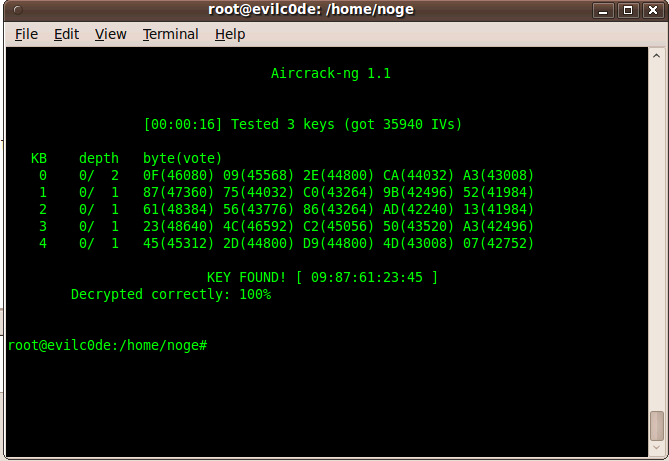
\includegraphics[width=0.9\textwidth]{images/WLAN/wepkey.png}
	 			\caption{WEP Schlüsselberechnung}
	 			\label{fig:WEP Schlüsselberechnung}
	 		\end{figure}

\subsection{Fazit}
Das WEP-Verschlüsselungsprotokoll ist heutzutage nicht mehr zeitgemäß. Es ist veraltet und unsicher egal in welcher Variante, weswegen man auch keine Router mehr finden sollte, die dieses Verschlüsselungsprotokoll verwenden. Dennoch findet man auch heute noch Router die WEP verwenden, auch wenn sie es nicht mehr sollten. Die Schlüssellänge verändert außerdem nur unwesentlich die Sicherheit von WEP. Abschließend lässt sich sagen, dass Wired Equivalent Privacy schnellstmöglich durch neuere Verfahren wie WPA2 ausgetauscht werden sollte, die die Sicherheit eher garantieren können.
\newpage

\section{WPA/WPA2}

WPA (WiFi Protected Access) ist die teilweise Implementierung des Sicherheitsstandards IEEE  802.11i für Funknetzwerke nach den WLAN-Standards IEEE 802.11a, b, g, n und ac. Ziel von WPA war es, nachdem die WEP-Verschlüsselung gebrochen wurde, rasch eine sichere Alternative zu bieten, die zudem kompatibel zur bereits auf dem Markt verfügbarer Hardware war. Die definierte Grundarchitektur für Schlüsselaustausch, Schlüsselgenerierung, Erneuerung des Schlüsselmaterials und Schutz der ausgetauschten Pakete von IEEE 802.11i wurde in WPA umgesetzt, allerdings wurden nicht die vom Standard vorgeschriebenen Algorithmen eingesetzt. Da WPA keine starken Krytographieverfahren unterstützt war es nur eine Frage der Zeit, wann auch dieses Verfahren geknackt wird. \\
Mit WPA2 erfolgte dann die vollständige Umsetzung von IEEE 802.11i. Im Gegensatz zu WPA verwendet WPA2 den Verschlüsselungsstandard Advanced Encryption Scheme (AES), wenn CCMP als Protokoll verwendet wird. WPA hingegen unterstützt nur die Stromchiffre RC4, die mit TKIP eingesetzt wird. \\
Die Implementierungen bestehen aus einer Kombination von Authentifizierung und Verschlüsselung, um ein WLAN sicher zu betreiben. Die Authentifizierung erfolgt entweder mit einem Passwort (Personal Mode), dem sogenannten Pre-Shared-Key (PSK), oder unter Verwendung eines RADIUS-Servers (Enterprise Mode), um den Zugriff durch unberechtigte Personen zu verhindern. \\

\subsection{WPA/WPA2 Personal Mode}
Im Personal Mode erfolgt die Netzwerk-Authentifizierung mit einem PSK, über den sowohl der Client als auch der Access-Point verfügen. Der PSK besitzt dabei eine Länge von 8 bis 63 Zeichen. Aus dem PSK berechnet sich der Pairwise Master Key (PMK) durch die Verwendung des Schlüsselableitungsverfahrens PBKDF2. Die Schwachstelle bei der PSK-Authentifikation ist der 4-Wege-Handshake der im nachfolgenden Abschnitt genauer beleuchtet wird.

\newpage
\subsubsection{Schwachstelle: 4-Wege-Handshake} \label{4wh}
Die Schwachstelle, welche bei Angriffen gegen WPA bzw. WPA2 ausgenutzt wird liegt im 4-Wege-Handshake der zur Authentifizierung durchgeführt wird. Der Handshake besteht aus folgenden Aktionen:
\begin{figure}[ht!]
	\centering
	
\includegraphics[width=0.5\textwidth]{images/WLAN/handshake.png}
	\caption{WPA/WPA2 4-Wege-Handshake (Quelle: kalitutorials.com)}
	\label{fig:WPA handshake}
\end{figure}

Wie in Grafik \ref{fig:WPA handshake} zu sehen, sendet bei einer Authentifikationsanfrage zuerst der Router (Access Point AP) eine Zufallszahl (ANonce) an den Client (STA). Dieser kann dann zusammen mit seiner Zufallszahl (SNonce) den Pairwise Transient Key (PTK) berechnen. Der PTK leitet sich aus dem PMK, den beiden Zufallszahlen aus dem Handshake und den MAC-Adressen ab. Dementsprechend berechnet er sich:

\begin{equation}
PTK = PMK + ANonce +SNonce  + MAC_{Client} + MAC_{AP}
\end{equation}

Anschließend sendet der STA nun noch seine SNonce zu, damit auch der AP den PTK berechnen kann. Zusätzlich schickt er ihm noch einen Message Integrity Code (MIC) mit, um Authentizität und Integrität zu gewährleisten. \\
Der PTK kann nun für die Verschlüsselung der Kommunikation zwischen Client und AP verwendet werden. Für eine Multicast-Kommunikation zwischen Client und anderen Clients wählt der AP einen zufälligen Group Master Key (GMK). Aus diesem leitet sich der Group Transient Key (GTK) ab, der wiederum an die Gruppenmitglieder verteilt wird. Falls ein Gruppenmitglied die Gruppe verlässt, müssen alle Nutzer die Schlüssel austauschen. \\
Zum Abschluss bestätigt der Client noch einmal dem AP die Kommunikation und schließt damit den 4-Wege-Handshake ab.\\
Angriffspunkt ist der MIC, welcher zur Integritätsprüfung mit übertragen wird. Dieser wird mit Hilfe des PMK berechnet. Der PMK wiederum wird vom PSK abgeleitet. Die Hashfunktion zur Berechnung des MIC kann bis heute nicht gebrochen werden, weshalb nur mittels Bruteforcing oder Wörterbuchangriff eine Übereinstimmung gefunden werden kann. Ist der PMK erfolgreich extrahiert, muss erneut per Bruteforcing/Wörterbuchangriff eine Übereinstimmung gefunden werden.

\subsubsection{Cracking des WPA/WPA2 PSK}
 Möchte ein Angreifer nun in das Netzwerk eindringen, muss er dieses Passwort herausfinden. Grundsätzlich gibt es beim Hacken keine Unterschiede zwischen WPA- und WPA2-gesicherte WLANs. Es ist immer das Ziel einen vollständigen 4-Wege-Handshake  aufzuzeichnen, aus dem dann das Passwort extrahiert werden kann. Wie im Abschnitt zuvor angedeutet erfolgt dies mit Hilfe von Bruteforcing oder einer sogenannten Wörterbuch-Attacke (engl. dictionary-attack). Bei Ersterem werden einfach alle Kombinationen bestehend aus Buchstaben, Ziffern und Sonderzeichen, oder nur einem Ausschnitt davon, bis zur gewünschten Länge auf Übereinstimmung getestet. Je nach Länge und Komplexität des Passworts kann sich dieser Vorgang über viele Stunden, bis zu Tagen und sogar mehreren Jahren hinziehen, da die Anzahl der möglichen Kombinationen exponentiell zur Länge des Passworts zunimmt. Häufig wird deshalb vor einer Bruteforce-Attacke eine Wordlist, wie bei einem Dictionary-Angriff, mit allen zu testenden Kombinationen erstellt. Bei einem Wörterbuch-Angriff wird somit durch die Passwortkandidaten in einer riesigen Wordlist iteriert und mit dem herauszufindenden Passwort abgeglichen. \\
Wörterlisten können entweder selber generiert werden oder sind auch im Internet zu finden. Wie  später noch zu sehen ist, gibt es auch hybride Ansätze, die beide Angriffsarten verknüpfen. Ein erfolgreicher Angriff steht und fällt mit einer guten Wordlist, in der das WLAN-Passwort enthalten sein muss/sein sollte). Darin besteht die eigentliche Schwierigkeit eines Angriffes auf ein WPA/WPA2-gesichertes WLAN. \\
Nachfolgend nun exemplarische eine Möglichkeit einen WPA/WPA2-PSK zu cracken:

\begin{enumerate}
	\item {Check des WLAN Adapter} \\
	Falls ein externer Adapter verwendet wir, muss folgendes beachtet werden. Zuerst muss geprüft werden, ob der eingesteckte USB oder der interne WLAN-Adapter richtig erkannt wird und somit einsatzbereit ist. Dazu muss das Terminal geöffnet und der Befehl \colorbox{altgray}{\lstinline|ifconfig|} eingegeben werden.

	Der Adapter sollte als Interface, meist wlan0 oder wlan1 (meist bei einem externen WLAN-Adapter), angezeigt werden. Im Folgenden muss bei allen Befehlen die Interface-Bezeichnung mit der hier Angezeigten ersetzt werden, da sie sich von Rechner zu Rechner abhängig von der Anzahl der installierten WLAN-Adapter unterscheiden kann.

	\item {Exkurs MAC-Spoofing} \\
Im Sinne von Wireless Security sollte man sich immer im Klaren sein, dass ein Angreifer immer in der Lage ist seine MAC-Adresse zu verändern, weswegen dieser Absatz hier zwar aufgeführt ist aber in den Versuchsskripten nicht genutzt wird. Dieser Vorgang wird auch Spoofing genannt. Die MAC-Adresse ist eine herstellerspezifische Kennung, die fest einem Netzwerkgerät zugeordnet ist. Jede Adresse ist eindeutig. Findet man die MAC-Adresse eines Angreifers heraus, kann mit Hilfe dieser Identifikationskennung festgestellt werden, welchen Typ von Antenne er verwendet. Diese Erkenntnis kann helfen einen Angreifer zu identifizieren. Verwendet ein Angreifer nun eine gefälschte MAC-Adresse können keine Rückschlüsse auf seine Identität gezogen werden, da überall nur seine Fake-Adresse angezeigt wird. Zuerst muss dafür das WLAN Interface deaktiviert werden. Danach kann mit dem Kommando \colorbox{altgray}{\lstinline|macchanger|} die Adresse geändert werden:\newline
	\newline
	\colorbox{altgray}{\lstinline|ifconfig wlanX down|}\newline
	\newline
	\colorbox{altgray}{\lstinline|macchanger -r wlanX|}\newline
	\newline
	wobei wlanX (auch in den folgenden Fällen) an das verwendete WLAN-Interface angepasst werden muss.\newline

	Beim Bestätigen des Befehls, wird die eigene MAC-Adresse in eine zufällige generierte MAC-Adresse geändert und auf der Konsole angezeigt. Anschließend kann das Interface mit folgendem Befehl wieder aktiv gesetzt werden.

	\colorbox{altgray}{\lstinline|ifconfig wlanX up|}\newline
	\newline
	Mit dem Befehl: \newline

	\colorbox{altgray}{\lstinline|ifconfig wlanX|}\newline

	kann überprüft werden, ob die gespoofte MAC-Adresse auch aktiv ist.\newline
	Dieser Schritt wird im Vorführskript übersprungen.

	\item {Das Interface in den Monitor Mode versetzen} \\
	Damit mit dem WLAN Adapter Pakete aufgezeichnet werden können, muss sich der Adapter im Monitoring Mode, oder auch Packet Injection Mode genannt, befinden. \\
	Dies wird mit folgendem Befehl erreicht:

	\colorbox{altgray}{\lstinline|airmon-ng start wlanX|}\newline

	Mit dem Befehl \newline
	\colorbox{altgray}{\lstinline|airmon-ng check kill|}\newline \newline
	werden alle andere Prozesse beendet, die auch auf den Netzwerkadapter zugreifen können. So können Konflikte beim Zugriff auf die Ressource vermieden werden.\newline

	\item {Aufzeichnen der WLAN Pakete mit \colorbox{altgray}{\lstinline|airodump-ng|}}\\
	Im nächsten Schritt werden die WLAN Pakete aus der Umgebung aufgezeichnet. Damit möchte man einen Handshake zwischen dem zu hackenden Access Point und einem Client aufzeichnen. Anhand dessen kann anschließend das Passwort herausgefunden werden. Der Name des WLANs ändert sich hier für gewöhnlich es ist also eine weitere Runde mit \colorbox{altgray}{\lstinline|ifconfig|} sinnvoll, um sicherzustellen, dass man den korrekten WLAN-Namen verwendet. Mit dem folgenden Befehl können wir nun in den Aufzeichnungsmodus umschalten: \newline

	\colorbox{altgray}{\lstinline|airodump-ng -b a wlanXmon|}\newline

	\begin{itemize}
		\item \bashCommand{-b a} Führe den Scann im 5 GHz Band durch
	\end{itemize}

	Sollten keine Daten aufgezeichnet werden, dann sollte der Adapter mehrmals aus- und wieder eingesteckt werden. Nach einem Reconnect muss der Adapter natürlich wieder in den Monitoring Modus versetzt werden. Hat alles soweit geklappt, sollten alle erreichbaren SSIDs mit ihren jeweiligen Sendern angezeigt werden. Als nächstes sollte die MAC-Adresse und der verwendete Kanal des zu hackenden APs, sowie die SSID notiert werden. Anschließend kann durch einen neuen \colorbox{altgray}{\lstinline|airodump-ng|} Durchlauf mit der MAC und dem Kanal als Parameter (nähere Infos unter \colorbox{altgray}{\lstinline|man airodump-ng|} abrufbar) der Scann eingeschränkt werden. Zusätzlich kann auch der Name der Ausgabedatei festgelegt werden. Der Befehl sieht dann in etwa wie nachfolgend aus:\\
	\\
	\colorbox{altgray}{\lstinline|airodump-ng -c Kanal -b a --bssid BSSID --showack -w Filename wlanXmon|} \\

	\begin{itemize}
		\item \bashCommand{-c} Kanal des Ziels angeben
		\item \bashCommand{-b a} Führe den Scann im 5 GHz Band durch
		\item \bashCommand{--bssid} BSSID (MAC) des Ziels angeben
		\item \bashCommand{--showack} Erweiterte Ausgabe bezüglich ACKs
		\item \bashCommand{-w} Prefix für die Ausgabedatei angeben (z. B. SSID des Ziels)
	\end{itemize}


	Verbindet sich nun ein Client auf den AP, so kann der 4-way-handshake mitgelesen werden, was auch in der Konsole, in der rechten oberen Ecke, angezeigt wird. Hat dies funktioniert, ist der erste Schritt für das Hacken des Passworts abgeschlossen. Um diesen Vorgang zu beschleunigen, kann mithilfe von \colorbox{altgray}{\lstinline|aireplay-ng|} ein Verbindungsabbruch eines Clients erzwungen werden, wodurch dieser sich erneut mithilfe eines 4-way-handshakes verbinden muss. Dazu wird folgender Befehl verwendet:\newline\newline

	\colorbox{altgray}{\lstinline|aireplay-ng --deauth 100 -a router_bssid wlanXmon|} \\

	\begin{itemize}
		\item \bashCommand{--deauth} Attackmode Deauth auswählen, mit Anzahl der zu sendenden Pakete
		\item \bashCommand{-a} Angabe der BSSID
	\end{itemize}


	\item Cracken des Passworts \\
	Zum Cracken des Passworts werden nachfolgend zwei Tools verwendet und vorgestellt.
	\end{enumerate}

	\subsubsection{Cracken des Passwortes mittels aircrack-ng}
	\begin{enumerate}
	\item Dictionary Attacke mit \colorbox{altgray}{\lstinline|aircrack-ng|} \\
	Dazu wird ein Dictionary File mit allen Passwörtern benötigt, die auf Übereinstimmung mit dem PSK gecheckt werden sollen. Im Projekt-Verzeichnis sollte bereits ein Beispiel-Dictionary mit den Passwörtern der Vorführgeräte vorbereitet sein. Mit folgendem Befehl kann der Dictionary-Angriff gestartet werden:

	\colorbox{altgray}{\lstinline|aircrack-ng -w dict.file -b BSSID File.cap|}\newline
	\begin{itemize}
		\item \bashCommand{-w} Angabe des Dictionarys
		\item \bashCommand{-b} Angabe der BSSID des Ziels
	\end{itemize}

	\item Brutefore Angriff mit \colorbox{altgray}{\lstinline|aircrack|} und \colorbox{altgray}{\lstinline|crunch|}\\
	\\
	\colorbox{altgray}{\lstinline|crunch 8 12 abcdeABCDE {|} aircrack-ng --bssid BSSID -w- hack-wifi-01.cap|}\newline
	\begin{itemize}
		\item \bashCommand{8 12} Minimale und Maximale Passwortlänge
		\item \bashCommand{abcdeABCDE} Verwendete Zeichen
		\item \bashCommand{--bssid} Angabe der BSSID des Ziels
		\item \bashCommand{-w} Pfad zur Wordlist (- steht dabei für die Standardeingabe)
	\end{itemize}
	\end{enumerate}

	\subsubsection{Cracken des Passwortes mittels hashcat}
	Bei \colorbox{altgray}{\lstinline|hashcat|} handelt es sich wohl um den derzeit schnellsten Passwortcracker auf dem Markt. Wir verwenden ihn als Alternative zu \colorbox{altgray}{\lstinline|crunch|}. Das Entschlüsseln mit \colorbox{altgray}{\lstinline|hashcat|} wird in den beiliegenden Versuchsskripten nicht verwendet. \colorbox{altgray}{\lstinline|Hashcat|} verwendet die GPU, was bei Notebooks und virtuellen Umgebungen zu Problemen führt. Der Vollständigkeit wegen wurde \colorbox{altgray}{\lstinline|hashcat|} dennoch aufgeführt und kann bei Interesse mit den nachfolgenden Befehlen getestet werden, wenn die verwendete Grafikkarte mit \colorbox{altgray}{\lstinline|hashcat|} kompatibel ist. Wichtig ist auch, dass eine dedizierte Grafikkarte benötigt wird. Mit dem nachfolgendem Befehl wir die cap-Datei in eine hccap-Datei umgewandelt, was der erste Schritt zur Nutzung von \colorbox{altgray}{\lstinline|hashcat|} ist.\newline
	\\
	\colorbox{altgray}{\lstinline|aircrack-ng Filename.cap -J newFilename|}\newline
	Filename.cap = Pfad bzw. Name des alten .cap files\newline
	Pfad bzw. Name des neuen .hccap file\newline\newline
	Mit \colorbox{altgray}{\lstinline|hashcat --help|} kann eine Hilfeseite aufgerufen werden in welcher der Befehl, die Parameter und die Verwendung genauer erläutert werden. Falls Probleme auftreten oder detailliertere Einstellungen vorgenommen werden sollen, kann die Hilfeseite die erste Anlaufstelle sein.
	\begin{enumerate}

	\item Dictionary-Attacke mit \colorbox{altgray}{\lstinline|hashcat|}

	\colorbox{altgray}{\lstinline|hashcat -m 2500 capture.hccap dict.txt|}\newline
	-m 2500 = Anweisung, dass ein WPA/WPA2 Key gecrackt werden soll\newline
	caputre.cap = Pfad bzw. Name des hccap file\newline
	dict.txt = Pfad bzw. Name des dictionary file

	Anschließend wird das Dictionary genutzt, um das Passwort zu finden. Mit Enter kann der aktuelle Status des Vorgangs abgefragt werden.
	\\
	\item Bruteforce-Attacke mit \colorbox{altgray}{\lstinline|hashcat|}

	\colorbox{altgray}{\lstinline|hashcat -m 2500 -a3 capture.hccap ?d?d?d?d?d?d?d?d (?d = 0-9)|}\newline
%	\begin{itemize}
%		\item \bashCommand{-m 2500} Art des Hashes (2500 für WPA/WPA2)
%		\item \bashCommand{-a3} Verwende Bruteforce \newline
%		\item \bashCommand{?d..?d} Definierte Maske fuer zu testenden Passwortkandidaten, Anzahl entspricht "`bis zu Länge'\newline
%		\begin{itemize}
%			Weitere Optionen:\newline
			%\item \bashCommand{?l} abcdefghi...yz\newline
			%\item \bashCommand{?u} ABCDEFGHI...YZ\newline
			%\item \bashCommand{?s} Sonderzeichen\newline
			%\item \bashCommand{?a} ?l?u?s?\newline
	%	\end{itemize}
%	\end{itemize}

	Bei der Bruteforce Attacke werden alle Kombinationen von Buchstaben bis zu einer bestimmten Länge getestet. Als letzter Parameter kann eine Art Maske angegeben werden, mit welcher die Länge und die zu testenden Ziffern, Buchstaben und Zeichen festgelegt werden. Im Beispiel werden alle bis zu neun stelligen Zahlenkombinationen von \colorbox{altgray}{\lstinline|hashcat|} durchprobiert.\newline

	\item rule-based Attacke mit \colorbox{altgray}{\lstinline|hashcat|}

	\colorbox{altgray}{\lstinline|hashcat -m 2500 -r /usr/share/hashcat/rules/best64.rule capture.hccap dict.txt|}\newline
	\begin{itemize}
		\item \bashCommand{-m 2500} Art des Hashes (2500 für WPA/WPA2)\newline
		\item \bashCommand{-r} Verwende rule-based Angriff und anschließende Pfadangabe\newline
    \end{itemize}
	Rule-based Attacken gehören zu den komplizierteren Angriffsarten. Dabei wird ein normaler Dictionary-Angriff gefahren, aber mit Regeln erweitert. Die Regeln sind wie eine Art Programmiersprache für die Generierung von Passwörtern. Es gibt Funktionen mit denen Passwortkandidaten bearbeitet, mit anderen Wörtern verknüpft oder bestimmte Kombinationen übersprungen werden können. Regeln zu schreiben kann sehr aufwändig sein und erfordert viel Wissen über Passwörter. Daher kann für die ersten Versuche auch die \colorbox{altgray}{\lstinline|best64.rule|} Regel verwendet werden, die standardmäßig bei \colorbox{altgray}{\lstinline|hashcat|} dabei ist.\newline
\end{enumerate}

\subsection{Enterprise Mode}
Der Enterprise-Mode wird in den meisten Fällen in Unternehmen eingesetzt. Falls hier ein Client Verbindung mit dem AP herstellt, sperrt der AP erst einmal die Nutzung des WLANs und lässt nur Authentifizierungsverkehr durch. Nun muss sich der Client mittels EAP authentifizieren. Ist diese Authentifizierung erfolgreich, dann geschieht die Schlüsselverteilung wie oben im Personal-Mode vorgestellt.\\
WLAN-Netze im Enterprise-Mode benutzen das Extensible Authentication Protocol (EAP). Es gibt verschiedenste Implementierungen dieses Protokolls. Eine sehr weit verbreitete Implementierung ist PEAP (Protected EAP). Diese wird auch im kommenden Angriffstutorial genutzt.

\subsubsection{Schwachstelle: Challenge-Response-Verfahren}
Um einem Nutzer Zugang zum Netz zu gewähren erhält dieser während des Verbindungsaufbaus eine Zufallszahl vom AP/RADIUS-Server als Challenge. Diese wird dann zusammen mit dem Passwort, das sowohl Server als auch Client bekannt ist, gehasht und an den Server zurück übertragen. Dieser prüft den Hash zu ein erneutes Berechnen und gewährt bei Übereinstimmung Zugang zum Netz. \\
Versucht nun ein Angreifer Zugang zum Netz zu erhalten, versucht er valide Credentials eines Netzteilnehmers zu knacken. Hierzu muss ein zweiter Hostspot (im weiteren Fake-AP bezeichnet), der unter der Kontrolle des Angreifers ist, aufgesetzt werden der identisch zum Originalhotspot ist. Wenn nun ein Client fälschlicherweise den Fake-AP für ein Original hält und einen Verbindungsaufbau startet, schickt der Angreifer eine Challenge und erhält eine Response. Aus dieser kann dann mittels eines Wörterbuch-Angriffs das Passwort der Clients extrahiert werden. \\
Die Verwechslung der APs kann aber dadurch ausgeschlossen werden, dass Clients die vom AP zur Verfügung gestellten Zertifikate auf Validität überprüfen. In Realität ist diese Funktion aber vor allem bei Mobilgeräten oftmals deaktiviert, weil hierzu erst das Serverzertifikat in das Gerät importiert werden muss.

\subsubsection{Cracking eines WPA/WPA2-Netzes im Enterprise Mode}
Um die Zugangsdaten eines Nutzers eines Enterprise-Mode WLANs zu erhalten, muss ein Fake-AP mit denselben Daten wie ein Original-AP in Reichweite von Clients platziert werden. Dieser AP sollte idealerweise die Originale an Signalstärke übertreffen, um Verbindungsversuche von Clients zu provozieren.
\begin{enumerate}
	\item {Installation eines Enterprise RADIUS-Servers} \\
	\textit{HINWEIS: Dieser Schritt ist nur durchzuführen, falls das Tutorial entweder außerhalb der Security-Workbench ausgeführt wird, oder im Unterverzeichnis \colorbox{altgray}{\lstinline|WIFI/|} der Workbench kein Verzeichnis \colorbox{altgray}{\lstinline|hostapd-X.X/|} existiert.} \\
	Für die Installation der RADIUS-Server-Software wurde das Skript \\ \colorbox{altgray}{\lstinline|Enterprise-ServerInstall.sh|} im Verzeichnis \colorbox{altgray}{\lstinline|WIFI/|} abgelegt. Diese Skript installiert neben wenigen Libraries den Deamon \colorbox{altgray}{\lstinline|hostapd|}. Dieser implementiert einen RADIUS-Authentifizierungsserver.\\
	Falls es zu Problemen bei der Installation des \colorbox{altgray}{\lstinline|hostapd|}-Deamons kommt, können auch die Archive mit der Kennzeichnung \colorbox{altgray}{\lstinline|_Enterprise|} entpackt werden und die benötigten Libraries (\colorbox{altgray}{\lstinline|libssl-dev libnl-3-dev|} und \colorbox{altgray}{\lstinline|libnl-genl-3-dev|}) per \colorbox{altgray}{\lstinline|apt-get install|} installiert werden.
	\item {Information Gathering}\\
	Um einen Fake-AP aufzusetzen, der Nutzern eines Enterprise-Netzes vortäuscht ein echter AP dieses WLAN-Netzes zu sein, muss ein Original-AP so gut wie möglich kopiert werden. Hierzu werden Informationen bzgl. SSID, Kanalnummer und angewendete WPA-Verfahren benötigt. Diese können mit dem Befehl  \colorbox{altgray}{\lstinline|airodump-ng [wlanX]|} ermittelt werden. Der Adaptername \colorbox{altgray}{\lstinline|wlanX|} sollte zuvor per \colorbox{altgray}{\lstinline|ifconfig|} abgefragt werden, falls noch nicht bekannt.
	\item {Manipulation der Interfaces-Konfiguration}\\
	Nachdem alle benötigten Informationen gesammelt sind, kann mit dem eigentlichen Angriff begonnen werden. Zuerst muss die Interfaces-Datei des Betriebssystems so angepasst werden, dass die Steuerung des WLAN-Adapters an den Netzwerkmanager delegiert wird: \\
	In der Datei \colorbox{altgray}{\lstinline|/etc/network/interfaces|} muss folgende Zeile hinzugefügt oder angepasst werden: \colorbox{altgray}{\lstinline|iface wlanX inet manual|}
	\item {Konfiguration des RADIUS-Servers}\\
	Sobald die Interfaces-Konfiguration abgeschlossen ist, muss in der Datei \colorbox{altgray}{\lstinline|hostapt-wpe.conf|} die RADIUS-Server-Konfiguration angepasst werden. Die Konfigurationsdatei befindet sich im Unterverzeichnis \colorbox{altgray}{\lstinline|WIFI/|} unter \colorbox{altgray}{\lstinline|hostapd-X.X/hostapd/|}.\\
	Folgende Anpassungen müssen erfolgen: \\
	\begin{itemize}
		\item Zeile 11: \colorbox{altgray}{\lstinline|interface=wlanX|}, wobei \colorbox{altgray}{\lstinline|wlanX|} durch den korrekten Adapternamen ersetzt werden muss.
		\item Zeile 14: Auskommentieren der Zeile \colorbox{altgray}{\lstinline|driver=wired|}, da ein WLAN-Interface genutzt wird.
		\item Zeile 25: Anpassen der SSID des Fake-AP unter \colorbox{altgray}{\lstinline|ssid=[AP-SSID]|}
		\item Zeile 27: Anpassen des Kanals des Fake-AP unter \colorbox{altgray}{\lstinline|channel=[Kanal-Nummer]|}
		\item Zeile 49: Anpassen der verwendeten WPA-Version des Fake-AP unter \colorbox{altgray}{\lstinline|wpa=[1 für WPA oder 2 für WPA2]|}
	\end{itemize}
	\item {Starten des Fake-AP}\\
	Da nun alle Konfigurationen erfolgt sind, kann der Fake-AP in Betrieb genommen werden und auf die ersten Opfer gewartet werden. Der Fake-AP lässt sich komfortabel mit dem Skript \colorbox{altgray}{\lstinline|startFakeAP.sh|} gestartet werden. Dieses startet den hostapd-Deamon mit der zuvor festgelegten Konfiguration. Bei jedem Authentifikationsversuch wird nun auf der Konsole die gesendete Challenge und erhaltene Response ausgegeben.
	\item {Cracken des Passwortes}\\
	Um nun aus der aufgenommenen Challenge und Response das Passwort zu extrahieren, muss ein Bruteforce- oder Wörterbuch-Angriff durchgeführt werden. \\
	Ein Wörterbuch-Angriff kann beispielsweise mittels \colorbox{altgray}{\lstinline|asleap|} erfolgen: \\
	\colorbox{altgray}{\lstinline|asleap -C [challenge] -R [response] -W [Dictionary-Datei]|}\\
	\textit{Hinweis:} Es kann zu einer Umcodierung der Wörterbuchdatei kommen, falls diese mit einem graphischen Texteditor wie Leafpad geöffnet wird. Änderungen an den Wörterbuchdateien sollten aus Kompatibilitätsgründen daher im Idealfall in der Konsole bspw. per \colorbox{altgray}{\lstinline|nano|} oder \colorbox{altgray}{\lstinline|vi|}  erfolgen.
\end{enumerate}


\subsection{Fazit}
Mit WPA wurde schnell eine Alternative zu WEP geboten, die aber auf Kompatibilität fokussiert war. Erst mit WPA2 kam durch die zwingende Verwendung komplexer Kryptoalgorithmen die gewünschte Sicherheit. \\
Grundsätzlich sind jedoch beide Verfahren nur so sicher, wie die verwendeten PSKs. Mit ausreichend langer Ausdauer eines Angreifer kann also der PSK des Netzes extrahiert werden. \\
Bei der Verwendung von WPA/WPA2 im Enterprise-Mode sollte besonders auf sichere Passwörter geachtet werden. Hier kann ein Angreifer nicht nur Zugang zum Netz erhalten, sondern kann sich auf bei eventuell im Netz laufenden Diensten anmelden. Wenn ein Client sich fälschlicherweise mit einem Fake-AP verbindet kann ein Angreifer auch hier mit entsprechendem Zeitaufwand die Zugangsdaten erhalten.
\newpage

\section{WPS}

WPS (Wi-Fi Protected Setup) ist ein Standard zum Verbindungsaufbau mit einem WLAN. Das Ziel von WPS ist es, das Hinzufügen von Geräten in ein bestehendes Netzwerk zu vereinfachen. Die oft komplexere Vorgehensweise anderer Verfahren und Standards soll so umgangen werden, ohne auf ausreichende Sicherheit zu verzichten. \\
Die grundlegende Funktionsweise von WPS lässt sich auf drei primäre Ansätze darstellen: Push-button Methode, Pin-Eingabe und NFC (Near Field Communication). Push-button ist die vorgeschriebene Variante, die anderen beiden Möglichkeiten sind optional, sind aber nicht auf allen Geräten verfügbar. \\
Die Varianten werden hier näher beschrieben:

\begin{itemize}
	\item Push-butten Konfiguration: Bei der Push-button Variante wird mit einem Knopfdruck für eine bestimmte Zeit Zugang zu einem WLAN ermöglicht. Zu diesem Zeitpunkt können sich alle Geräte die sich in Reichweite des WLANs befinden verbinden. Der Knopf muss nicht unbedingt physischer Natur sein sondern kann auch softwareseitig sein. Das gerade hier Probleme auftreten können, in Gebieten wo sich viele WLAN-fähige Geräte befinden muss wohl nicht extra erwähnt werden.

	\item PIN Eingabe: Bei dieser Variante wird vom WLAN-Router ein Pin bereitgestellt mit dem sich ein Gerät im WLAN anmelden kann. Es ist sowohl möglich, dass dynamisch vom Gerät ein Pin bereitgestellt wird oder, dass ein einzigartiger Pin vom Router bereitgestellt wird. Der Pin soll problematische Verbindungen verhindern und eine zusätzliche Sicherheit bieten damit sich nicht einfach jedes Gerät in Reichweite verbinden kann, sollte die Push-button Methode angewendet werden. Wie der Authentifizierungsprozess des Pin-Verfahrens genau funktioniert wird später erklärt.

	\item Near Field Communication (NFC): NFC kann genutzt werden ohne eine manuelle Eingabe ein Gerät in ein WLAN aufzunehmen. Hier muss sehr intensiv darauf geachtet werden, dass Sicherheitsmaßnahmen getroffen werden, damit sich nicht unbekannte oder gefährliche Geräte mit dem WLAN verbinden.
\end{itemize}

\subsection{Authentifizierung per Pin-Eingabe}

Die Authentifizierung per WPS-Pin sieht die Eingabe einer acht stelligen Zahlenfolge auf dem WLAN-Client vor. Hiermit kann eine mögliche sehr komplexe WPA-Passworteingabe vermieden werden. Die WPS-Pin-Methode sieht vor, dass das WLAN-Passwort dem WLAN-Client mitgeteilt wird, wenn eine korrekte WPS-Pin eingegeben wurde. Dabei übermittelt der WLAN-Router dem Client ein Einrichtungspaket mit dem WLAN-Passwort, also dem WPA/WPA2 Schlüssel. \\
Folgender Vorgang zeigt den Ablauf einer Authentifizierung bei der WPS-Pin-Eingabe:

\begin{enumerate}
	\item Der WLAN-Client bittet den WLAN-AP um eine WPS-Pin-Authentifizierung.
	\item Anschließend tauschen beide den Schlüssel für die Transport-Verschlüsselung per Diffie-Hellman aus.
	\item Die Authentizität des WLAN-APs muss vom Client geprüft werden, weil sich ein fremder AP die Pin abgreifen könnte. Das heißt, der Client muss sicherstellen, dass er mit dem richtigen AP die WPS-Authentifizierung durchläuft und nicht mit einem AP, der zufällig den gleichen Namen hat.
	\item Der AP packt je eine vierstellige Pin-Hälfte (mit Zufallszahl gehasht), der insgesamt achtstelligen Pin, in einen verschlüsselten Container und schickt sie an den WLAN-Client. Der kann damit allerdings noch nichts anfangen.
	\item Der Client schickt jetzt die erste Hälfte seiner Pin transportverschlüsselt an den AP.
	\item Wenn dieser erste Teil der Pin korrekt ist, dann schickt der AP die Zufallszahl für die erste Pin an den Client.
	\item Der Client kann daraufhin die erste Pin (mit Zufallszahl gehasht) verifizieren. Er weiß dann, ob er mit dem richtigen AP verbunden ist.
	\item Dann schickt der Client die zweite Hälfte seiner Pin transportverschlüsselt an den AP.
	\item Wenn auch der zweite Teil der Pin korrekt ist, dann bekommt der WLAN-Client vom AP die zweite Zufallszahl und das WLAN-Passwort.
	\item Mit der zweiten Zufallszahl verifiziert der Client auch den zweiten Teil der Pin, die er vom AP bekommen hat.
	\item Wenn diese korrekt ist erfolgt die Anmeldung mit dem WLAN-Passwort per WPA/WPA2.
\end{enumerate}

\subsection{Schwächen von WPS}

Das Aktivieren der WPS-PIN-Methode im Access Point führt bei vielen Modellen dazu, dass ein fremdes Gerät über eine Brute-Force-Methode innerhalb weniger Stunden eine Verbindung herstellen kann und somit auch den Sicherheitsschlüssel unabhängig von dem verwendeten Verschlüsselungsverfahren erhält. \\
Durch einen verbreiteten Fehler in der Implementierung ist es dabei oft nur nötig, eine vierstellige sowie eine dreistellige PIN zu erwürfeln, was die Zahl der Möglichkeiten deutlich verringert. Bei einer Verbindung mittels WPS kann nahezu unmittelbar nach Herstellung der Verbindung das zum Access Point gehörige Wi-Fi-Passwort als Klartext ausgelesen werden. Es ist daher ratsam, die Funktion nicht oder nur als letzte Möglichkeit zu aktivieren, die Anmeldung des Geräts zu prüfen und WPS danach wieder abzuschalten. Nach der Anmeldung sollte auf Anzeichen von unbefugtem Zugriff auf das Netzwerk geachtet und gegebenenfalls das Wi-Fi-Passwort neu gesetzt werden. \\
Bei einigen der betroffenen Access Points ist die WPS-Funktion, obwohl sie in den Einstellungen deaktiviert wurde, weiterhin aktiv. Außerdem bieten auch einige ältere Modelle die Möglichkeit einen Pin selbst zu bestimmen was ebenfalls problematisch sein kann wenn man einen zu einfachen Pin wählt.

\subsection{Cracking des WPS-Schlüssels}
Folgender Vorgang soll den Ablauf des Hackvorgangs beim WPS-Verfahren zeigen:

\subsubsection{Check des WLAN-Interfaces}
	Falls ein externer Adapter verwendet wir, muss folgendes beachtet werden. Zuerst muss geprüft werden, ob der eingesteckte USB WLAN-Adapter erkannt wird und somit einsatzbereit ist, falls dieser verwendet wird. Dazu muss das Terminal öffnen in Kali Linux öffnen und den Befehl \colorbox{altgray}{\lstinline|ifconfig|} eingeben.

	Der Adapter sollte als Interface, meist WLAN0 oder WLAN1 (meist bei einem externen WLAN-Adapter), angezeigt werden. Im Folgenden muss bei allen Befehlen die Interface-Bezeichnung mit der hier angezeigten ersetzt werden, da sie sich von Rechner zu Rechner unterscheiden kann.

	\subsubsection{Das Interface in den Monitor Mode versetzen}
	Damit im WLAN Pakete aufgezeichnet werden können, muss sich die WLAN-Karte oder der Adapter im Monitor Mode befinden. \\
	Dies wird mit folgendem Befehl erreicht: \\
	\colorbox{altgray}{\lstinline|airmon-ng start wlanX|} \\

	Zusätzlich wird nach dem Versetzen in den Monitor Mode erneut der Name des WLAN-Adapters mit \colorbox{altgray}{\lstinline|ifconfig|} nachgesehen, da sich der Name des Adapters ändern kann. Mit dem Befehl \colorbox{altgray}{\lstinline|airmon-ng check kill|} werden zusätzlich alle laufenden Prozesse, die Probleme verursachen könnten, beendet.

	\subsubsection{Scannen der WLANs \colorbox{altgray}{\lstinline|airodump-ng|}}
	Im nächsten Schritt werden die WLAN Pakete aus der Umgebung aufgezeichnet. Damit möchte man einen Handshake zwischen dem zu hackenden Access Point und einem Client aufzeichnen. Anhand dessen kann anschließend das Passwort herausgefunden werden. Der Name des WLANs ändert sich hier für gewöhnlich es ist also eine weitere Runde mit \colorbox{altgray}{\lstinline|ifconfig|} sinnvoll, um sicherzustellen, dass man den korrekten WLAN-Namen verwendet. Mit dem folgenden Befehl können wir nun in den Aufzeichnungsmodus umschalten: \newline
	\colorbox{altgray}{\lstinline|airodump-ng -b a wlanXmon|}\newline
	\begin{itemize}
		\item Falls wir im im 5GHz Bereich scannen möchten muss der Parameter -b a mitgegeben werden. Falls nicht, kann der Parameter einfach weggelassen werden
		\item wlanXmon steht für die SSID des eigenen Adapters im Monitor Mode
	\end{itemize}

	 Sollten keine Daten aufgezeichnet werden, dann den Adapter mehrmals aus- und wieder einstecken. Nach einem Reconnect muss der Adapter natürlich wieder in den Monitoring Modus versetzt werden. Hat alles soweit geklappt, sollten alle erreichbaren SSIDs mit ihren jeweiligen Sendern angezeigt werden. Als nächstes sollte die MAC-Adresse und der verwendete Kanal des zu hackenden APs notiert.

	\subsubsection{Beginn des Angriffs mit \colorbox{altgray}{\lstinline|wash|} und \colorbox{altgray}{\lstinline|reaver|}}

	Zu Beginn des Angriffs muss getestet werden, ob der Zielrouter WPS unterstützt. Dies wird mit folgendem Befehl erreicht: \\
	\colorbox{altgray}{\lstinline|wash -i wlanXmon -c KANAL -C -s|}\newline
		\begin{itemize}
			\item -s stellt den Scanner-Mode bei \colorbox{altgray}{\lstinline|wash|} ein
			\item -C werden Frame-Prüfsummenfehler ignoriert
			\item Mit -i wird der WLAN-Adapter spezifiziert
			\item -c stellt den da Zielkanal
		\end{itemize}


		Eine mögliche Ausgabe von  \colorbox{altgray}{\lstinline|wash|} zeigt folgende Abbildung:
				\begin{figure}[H]
					\centering
					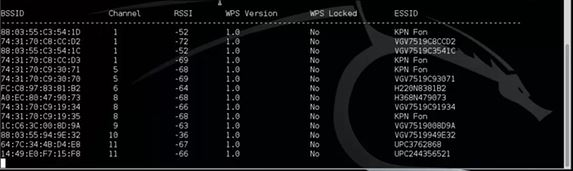
\includegraphics[width=0.9\textwidth]{images/WLAN/WashWPS.jpg}
					\caption{Wash Ausgabe}
					\label{fig:Wash Ausgabe}
				\end{figure}


	Nach der Ausgabe von \colorbox{altgray}{\lstinline|wash|} wird nun die WPS-PIN geknackt und der WPA2-PSK extrahiert mit dem Aufruf von \colorbox{altgray}{\lstinline|reaver|} der wie folgt lautet:
	\colorbox{altgray}{\lstinline|reaver -i wlanXmon -b BSSID|}
			\begin{itemize}
				\item -b spezifiziert hierbei das Ziel des Angriffs das zuvor durch \colorbox{altgray}{\lstinline|wash|}
				\item -i spezifiziert auch hier den WLAN-Adapter
			\end{itemize}

		Folgende Abbildung zeigt wie die Ausgabe aussieht. Das weiße Feld würde im optimalen Fall das Ergebnis enthalten.

						\begin{figure}[H]
							\centering
							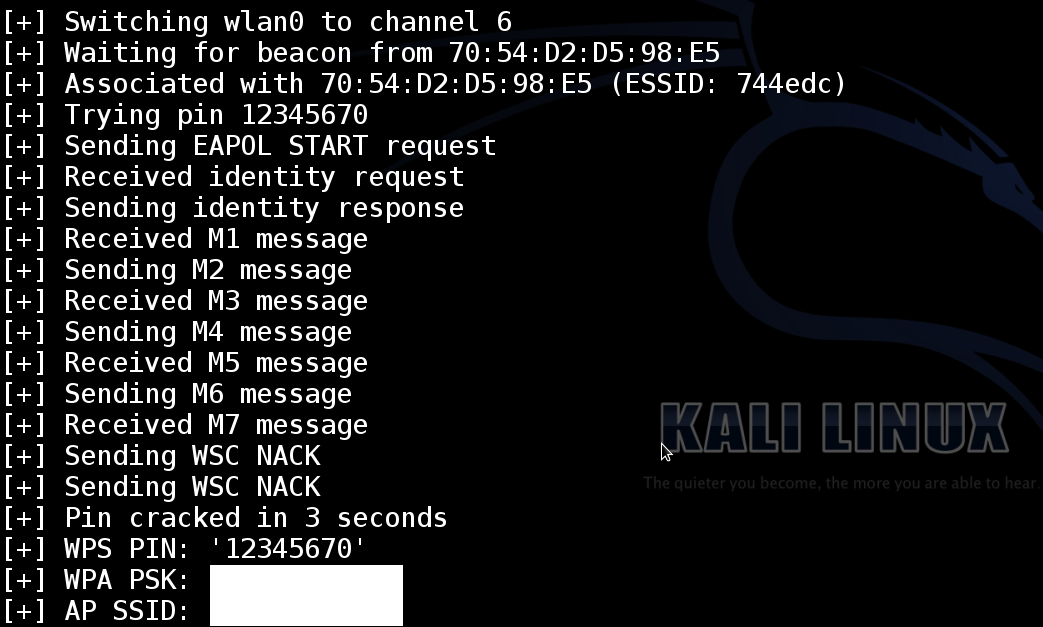
\includegraphics[width=0.9\textwidth]{images/WLAN/reaver.png}
							\caption{Reaver Ausgabe}
							\label{fig:Reaver Ausgabe}
						\end{figure}

	\subsubsection{Alternativer Angriff mit \colorbox{altgray}{\lstinline|bully|}}

	Alternativ zu \colorbox{altgray}{\lstinline|reaver|} bietet sich auch das Programm \colorbox{altgray}{\lstinline|bully|} an mit dem der Angriff durchgeführt werden kann. Wir starten den Vorgang mit folgendem Befehl: \\
	\colorbox{altgray}{\lstinline|bully wlanXmon --b BSSID -e SSID -c KANAL|}
				\begin{itemize}
					\item --b stellt die Ziel-Mac-Adresse da
					\item -c steht für den Kanal auf dem der Acces Point sendet
					\item wlanXmon steht für die SSID des eigenen Adapters im Monitor Mode
					\item -e der Name des Ziel-Access Points
				\end{itemize}

	Sollte das Ziel verwundbar sein für einen WPS-Angriff wird \colorbox{altgray}{\lstinline|bully|} das Passwort nach einiger Zeit ausgeben.

\subsection{Fazit}

WPS ist heute ohne Zweifel immer noch von Interesse, da es eine einfache Möglichkeit bietet Geräte in ein WLAN aufzunehmen ohne ihnen den möglicherweise sehr komplexen WPA-Schlüssel zu geben. Es bietet also einen vereinfachten Weg zusätzlich zu WPA. Daneben muss jedoch klar sein, dass nach der einfachen Push-button Methode immer überprüft werden muss, ob sich Geräte im WLAN befinden die dort nichts zu suchen haben. \\
Die Probleme früherer Geräte mit WPS, die unter dem obigen Kapitel aufgeführt wurden sind allerdings mittlerweile behoben. Einerseits wurden laufende Schlüsselwechsel eingeführt und andererseits wurde sichergestellt, dass der Zugang bei der push-button Methode zeitlich begrenzt ist. \\
\newpage

\section{DoS}
Ein Denail of Service-Angriff hat das Ziel, ein Netzwerk oder einen Server zu blockieren. Im Grunde basiert es einfach darauf durch eine Masse von Anfragen das Ziel zu überlasten und es im optimalen Fall zum Absturz zu bringen. Ein Erfolg ist hier also nicht Zugang zum Netz zu erhalten, sondern das Ziel möglichst lange in seinen Diensten einzuschränken, zu blockieren oder unbenutzbar zu machen. Dazu werden die zur Verfügung stehenden Programme oder Netzwerk-Ressourcen außerordentlich überbelastet, manchmal auch kollektiv von tausenden Nutzern. Große Ziele, also zum Beispiel Firmenserver die ohnehin starken Datenverkehr gewohnt sind, können nicht von einem einzigen eifrigen Angreifer mit seinem heimischen Computer in Bedrängnis gebracht werden. Außerdem wird an dieser Stelle darauf hingewiesen, dass hier von DoS-Angriffen die Rede ist, die von außerhalb des Ziel-WLANs erfolgen. DoS-Angriffe die in einem WLAN oder LAN erfolgen, werden an anderer Stelle bearbeitet. \\
Für den Angriff wird hier das Tool \colorbox{altgray}{\lstinline|MDK3|} (Murder Death Kill 3) verwendet, welches speziell für WLAN-Netzwerke entwickelt wurde. \\
Zuerst müssen auch hier wieder die um den WLAN-Adapter konkurrierenden Prozesse über das Kommando
\colorbox{altgray}{\lstinline|airmon-ng check kill|}
beendet werden.
Danach versetzen wir den WLAN-Adapter in den Monitoring-Modus. Dies geschieht über das Kommando:
\colorbox{altgray}{\lstinline|airmon-ng start wlanX|}.
Der WLAN-Adapter erhält hier für gewöhnlich einen neuen Namen mit der Form wlanXmon. Allerdings sei auch hier noch einmal darauf hingewiesen, dass sich der Name und eine mögliche Veränderung von System zu System unterscheiden kann.
\\
Anschließend suchen wir uns den Ziel-Access Point aus. Dies geschieht über den Befehl:
\colorbox{altgray}{\lstinline|airodump-ng wlanXmon --band abg|}. Aus der von diesem Werkzeug generierten Liste notieren wir die MAC-Adresse des Ziel-Access Points (BSSID) und die Art der Verschlüsselung. Diese Informationen werden im weiteren Verlauf benötigt.
\\
Das MDK3-Tool stellt verschiedene Methoden bereit, um einen DoS-Angriff auf dem Ziel auszuführen.

\subsection{Michael shutdown exploitation}
Diese Methode nutzt einen Fehler in der TKIP-Verschlüsselung aus, um den gesamten Datenverkehr im Ziel-Netzwerk zu unterbinden. Für einen erfolgreichen Angriff muss das WLAN mit TKIP verschlüsselt worden sein.\\
\colorbox{altgray}{\lstinline|mdk3 wlanXmon m -t BSSID -j|}. Durch den Parameter -j wird mdk3 angewiesen, eine Schwachstelle in der QoS-Implementierung der TKIP-Verschlüsselung auszunutzen. Dadurch werden nur ein paar Datenpakete benötigt, um den Datenverkehr zu blockieren. m steht für die Art des Angriffs hier also ein Angriff auf die TKIP-Verschlüsselung und versucht jeglichen Datenverkehr anhaltend zu stören. Mit -t wird das Ziel näher definiert.

\subsection{Beacon Flood Mode}
Bei dieser Methode werden Beacon-Frames ausgesendet, um den Clients gefälschte Access Points vorzugaukeln. Dies kann zu Abstürzen der Netzwerkscanner oder Treiber der WLAN-Adapter führen.
\colorbox{altgray}{\lstinline|mdk3 wlanXmon b -c KANAL|}
Der Parameter wlanXmon muss wieder durch den eigentlichen Namen des WLAN-Adapters ersetzt werden.
Das -c legt den Funkkanal fest, auf dem die Access Points erstellt werden sollen. b setzt hier wieder den Angriffsmodus da.

\subsection{Authentication DoS mode}
Bei dieser Methode werden vom Angreifer Authentication-Frames an den durch die BSSID spezifizierten Access Point geschickt. Zu viele Clients bringen den Access Point möglicherweise zum Absturz. Der Befehl
\colorbox{altgray}{\lstinline|mdk3 wlanXmon a -a BSSID|} führt den Angriff aus. a steht für den Angriffsmodus mit -a wird das Ziel näher definiert.

\subsection{Deauthentication DoS mode}
Bei diesem Angriff wird versucht jedem, der auf einem Access Point eingeloggt ist, den Zugang zu verwehren. Der Befehl \colorbox{altgray}{\lstinline|mdk3 wlanXmon d -b blacklist -c KANAL|} führt den Angriff aus. Das d steht hier für den Angriffsmodus, das -b blacklist ruft eine Liste der enthaltenen Angriffsziele auf, es ist auch das Nutzen von whitelists möglich. -c legt hier wieder den Kanal fest auf dem gesendet werden soll.

\subsection{Fazit}

Der Beacon Flood Mod konnte in den durchgeführten Versuchen keine Erfolge erzielen, während die anderen Angriffsmodi sich als zuverlässig erwiesen. DoS-Angriffe sind immer noch relevant und auch neuere Fritzboxen konnten durch die Angriffe zum Absturz gebracht werden.
\newpage

\section{Fake Access-Points}
Bereits beim Hacking von WPA/WPA2-Enterprise-Netzen wurde ein Fake-AP genutzt, um einen legitimen Netzwerkzugangspunkt zu imitieren.\\ Die Idee bösartiger WLAN-Zugangspunkte gibt es schon länger, doch diese Bedrohung gewinnt durch vermehrt aufgetauchte Skripte und Programme an Bedeutung. Für einen Fake AP wird meist ein Laptop so konfiguriert, das er sich als Hotspot oder Access Point ausgibt.\\ Dabei besteht entweder die Möglichkeit, eine bestehende SSID in der Umgebung zu wählen oder eine für viele Besitzer interessante SSID zu wählen. \\
Der Betreiber eines Fake-AP versucht in der Regel Informationen vom Opfer zu erlangen, beispielsweise über Phishing-Seiten. Auch ein Einschleusen von Schadcode auf dem Opfer ist möglich. \\
Ein bekanntes Tool um Fake-APs zum Phishing zu erstellen ist der \colorbox{altgray}{\lstinline|wifiphisher|}.

\subsection{Wifiphisher Installation}
\textit{HINWEIS: Dieser Schritt ist nur durchzuführen, falls das Tutorial außerhalb der Security-Workbench ausgeführt wird.}\\
Um die Installation so einfach wie möglich zu gestalten, steht im Unterverzeichnis \colorbox{altgray}{\lstinline|WIFI/|} der Security-Workbench das Installationsskript \colorbox{altgray}{\lstinline|wifiphisherInstalltion.sh|} zur Verfügung. Wurde dieses erfolgreich ausgeführt sind alle benötigten Tools installiert.

\subsection{Theoretischer Ablauf}

Zunächst wird ein eventuell vorhandener Access Point blockiert. \\
Im nächsten Schritt wird ein eigener Access Point beziehungsweise Hotspot erstellt. \\
Anschließend wird gewartet, bis sich Benutzer am Access Point anmelden. Ist das Signal des Angreifers aufgrund von z.B. örtlicher Nähe stärker, so kann es sein, dass sich die Opfer automatisch mit dem Fake Access Point verbinden. \\
Je nach Ziel des Angreifers wird den Opfern nun eine Anmeldemaske zum Phishing von Passwörtern oder Kreditkarten angezeigt.
Auch ein Mitlesen und die Manipulation des Datenverkehrs sowie eine Infektion des Opfers mit Schadcode über Lücken im Betriebssystem beziehungsweise im Browser ist möglich.

\subsection{Erstellen eines Fake-AP mit Wifiphisher}
In der Security-Workbench wird das Konsolen-Tool \colorbox{altgray}{\lstinline|wifiphisher|} gestartet.\\
Anschließend führt das Programm eine Suche nach WLANs in der Umgebung durch. Aus dieser Liste kann ein  Zielnetzwerk ausgewählt werden. Im Anschluss daran wird ein Webserver und der Fake AP mit der entsprechenden Konfiguration gestartet. \\
Danach wird begonnen, den Datenverkehr im Zielnetzwerk durch Abmeldung der Opfer vom Ziel-Access Point zu unterbrechen. \\
Das Opfer verbindet sich im Anschluss mit dem falschen Access Point des Angreifers, dieser befindet sich nun in einer "'Man in the Middle"'-Position. \\
Beim Aufruf einer Webseite wird dem Opfer nun eine Webseite präsentiert, die der Konfigurationsoberfläche des Routers nachempfunden ist und zur Eingabe des WLAN-Zugangskennwortes aufgrund eines durchgeführten Firmwareupdates auffordert. Denkbar ist auch die Nachbildung von Login-Seiten verschiedener sozialer Netzwerke oder Mailprovider. Auch die Fälschung von Login-Seiten für Hotspots ist möglich. \\
War der Angriff erfolgreich, das heißt ein Opfer hat beispielsweise das WLAN-Zugangskennwort auf der präsentierten Seite eingegeben, so beendet sich \colorbox{altgray}{\lstinline|wifiphisher|} nach dem Anzeigen der eingegebenen Daten.

\section{Gegenmaßnahmen}
Im nachfolgenden Kapitel werden kurz mögliche Gegenmaßnahmen beleuchtet, die oben vorgestellte Angriffe verhindern bzw. erschweren.
\subsection{WEP}
Der WEP-Standard gilt als nicht mehr sicher und ist durch WPA bzw. WPA2 abgelöst. Die einfachste Gegenmaßnahme um sich vor einem Angriff auf WEP zu schützen ist das Abschalten von WEP-gesicherten Netzen. Neuere Router bieten zwar die Möglichkeit von WEP-Absicherung, diese sollte aber auf keinem Fall mehr verwendet werden. \\
Falls man aus Kompatibilitätsgründen auf WEP angewiesen ist, sollte unbedingt geprüft werden, ob nicht auf neuere Hardware umgestiegen werden kann, da WEP keine Sicherheit mehr garantieren kann. Außerdem werden Versuche WEP sicherer zu machen, namentlich die Shared-Key-Authentication, eher als unsicherer betrachtet, da das Passwort hier mehrfach verwendet wird, wodurch es noch verfügbarer für Angreifer wird. \\
Die beste Gegenmaßnahme gegen Angriffe auf das WEP-Netz ist die Einfachste überhaupt: kein WEP verwenden.

\subsection{WPS}
WPS wird nach wie vor verwendet und effektive Gegenmaßnahmen sind in erster Linie moderne Hardware, da diese, wie bereits oben erwähnt, die Probleme älterer Geräte nicht mehr kennen und eine erheblich geringere Angriffsfläche liefern. \\
Lediglich das Verwenden des Push-Buttons ohne weitere Key Eingabe ist problematisch, da sich alle Geräte in Reichweite ohne weitere Sicherheiten einbinden können. Es sollte also nach jedem Nutzen des Push-Buttons geprüft werden, ob sich unbekannte Geräte im WLAN befinden. Befolgt man diesem Ratschlag ist auch der Push-Button verhältnismäßig sicher.

\subsection{WPA/WPA2}
Da WPA bzw. WPA2 in fast jedem Haushalt/Unternehmen eingesetzt wird, sind hier Gegenmaßnahmen zu den oben demonstrierten Angriffen besonders relevant.
\subsubsection{Personal-Mode}
Grundsätzlich sind jedoch beide Verfahren nur so sicher, wie die verwendeten PSKs. Jeder Nutzer sollte also Standardpasswörter der Auslieferung sofort ersetzen und möglichst die maximal mögliche Passwortlänge ausnutzen. Auch sollte der Key so zufällig wie möglich gestaltet werden. Nur dann kann mit hoher Wahrscheinlichkeit davon ausgegangen werden, dass das Netz sicher ist. \\
Viele Router bieten aktuell in der Standardkonfiguration WPA und WPA2 im Kombinationsbetrieb an. Der reine Einsatz von WPA2 sollte einem Kombibetrieb immer vorgezogen werden. \\
Beim Verwendung von WPA/WPA2 im Enterprise Mode sollte entweder von Administrator- oder Nutzerseite darauf geachtet werden, dass das verwendete Passwort zur Anmeldung ebenfalls möglichst viele Zeichen besitzt und einen hohen Grad an Zufall besitzt.
\subsubsection{Enterprise-Mode}
Im Enterprise-Mode gibt es eine sehr effiziente Möglichkeit das Verbinden zu einem Fake-AP zu verhindern bzw. zu vermeiden. Die RADIUS-Server stellen immer Zertifikate zur Verfügung, die bei einem Verbindungsversuch dem Client übermittelt werden. Wird nun von einen Fake-AP ein mit hoher Wahrscheinlichkeit nicht vertrauenswürdiges Zertifikat verwendet, wird dies bei der Prüfung entdeckt und kein Challenge-Response-Verfahren durchgeführt. Besonders in Mobilgeräten kann die Installation dieser Zertifikate aufwändig sein, sollte jedoch immer durchgeführt werden, um die Sicherheit der eigenen Credentials zu gewähren.
\subsubsection{Fake-Access-Points}
Bei dem Verbinden mit einem WLAN-Netz sollte immer darauf geachtet werden, ob das Netz so konfiguriert ist, wie die Verbindung in der Verbindungsstatistik des Betriebssystems dokumentiert ist. Die meisten Betriebssysteme warnen heutzutage auch davor, wenn versucht wird eine Verbindung zu einem WLAN mit bekannter SSID aufzubauen, welches aber eine abweichende Konfiguration aufweist. Bei einer solchen Verbindungswarnung sollte man nur mit äußerster Vorsicht eine Verbindung mit dem Netz aufbauen.
